\documentclass[11pt,a4paper]{article}
\usepackage[utf8]{inputenc}
\usepackage[T1]{fontenc}
\usepackage[french]{babel}
\usepackage[margin=2.5cm]{geometry}
\usepackage{hyperref}
\usepackage{graphicx}
\title{Université de Montpellier -- Faculté des Sciences\\[0.5em]
HAI913I -- Évolution et restructuration des logiciels\\[0.5em]
TP2 : Compréhension et architectures\\[0.5em]
\large Enseignant responsable : Bachar Rima\\Année universitaire 2026--2027}
\author{Alexandre SIREIX\\Numéro étudiant : 22414718\\Parcours : GL\\Rendu en monôme}
\date{8 novembre 2026}
\begin{document}
\begin{titlepage}
\maketitle
\thispagestyle{empty}
\end{titlepage}
\pagenumbering{roman}
\tableofcontents
\clearpage
\pagenumbering{arabic}

\section{Objectif et organisation}
Nous souhaitons transformer les faits du TP1 en modules candidats : couplage,
graphe pondéré, regroupement hiérarchique, dendrogramme et coupe sous contraintes.
Les parties A0 à B4 sont réalisées, ainsi que les bonus C1, C2 et C3.
Le bonus C4 n'est pas réalisé, faute de second projet Java disponible.
Le projet Maven du TP1 est repris dans le dossier \texttt{source/} du TP2.

\subsection{Informations de remise}
Ce travail est rendu en monôme par Alexandre SIREIX (22414718, parcours GL),
avec une date de remise prévue le 8 novembre 2026.
Le dépôt du projet est :
\href{https://github.com/ASireix/HAI913ITP2}{github.com/ASireix/HAI913ITP2}.
La vidéo de démonstration est accessible à l'adresse
\href{https://youtu.be/EB8bpRMm6iI}{youtu.be/EB8bpRMm6iI}.
Ces deux liens sont également regroupés dans \texttt{liens.txt}, à la racine
du dépôt. La remise utilise la vidéo externe, sans fichier vidéo dans l'archive.

\subsection{Architecture générale}
Le chemin principal réutilise notre extracteur TP1 : une analyse JDT produit
\texttt{ProjectFacts} et le graphe d'appel ; un adaptateur expose ensuite les
faits neutres au TP2. Le chemin CSV sert de comparaison et de micro exemple.
La chaîne de calcul ne connaît ni les AST ni les bindings.
\begin{center}
\fbox{\shortstack{Producteur TP1 ou CSV\\Classes, méthodes, arcs}}
$\longrightarrow$ \fbox{\shortstack{Couplage\\Graphe pondéré}}\\[1em]
$\longrightarrow$ \fbox{\shortstack{Clustering\\Dendrogramme}}
$\longrightarrow$ \fbox{\shortstack{Coupe CP\\Modules}}
\end{center}
La CLI et Swing sont deux interfaces de la même chaîne.
\begin{center}
\begin{tabular}{ll}
Objet & Relations principales du modèle \\
\hline
InputFacts & classes, propriétaires des méthodes, arcs \\
Coupling & classes et table des couples vers leur compte \\
WeightedGraph & sommets et arêtes pondérées \\
ClusteringService.Result & feuilles et liste chronologique des fusions \\
Dendrogram.Node & membres, similarité, fils gauche et droit \\
ModuleCut.Result & seuil, limite, modules et statut
\end{tabular}
\end{center}
Les collections exposées sont non modifiables. Les services de calcul sont
séparés du chargement, de l'affichage et des exports. Le code cible Java 17 ;
l'environnement utilisé est Windows 11, Amazon Corretto 17.0.13 et Maven 3.10.0.
Les dépendances Java sont JDT Core 3.46.0 et JUnit Jupiter 5.14.4 pour les tests.
Graphviz 16.1.0 via \texttt{@viz-js/viz} 3.31.0 sert uniquement aux images.

\subsection{Conventions de référence}
Nous comptons les arcs de méthodes internes au projet, sans les sites répétés,
et écartons les arcs intra-classe du couplage. Le dénominateur est le nombre
global d'arcs inter-classes. La référence utilise le lien moyen, le départage
lexicographique sur identifiants stables et une tolérance de $10^{-9}$ pour les
égalités de fusion. La coupe utilise une moyenne interne strictement supérieure
à CP, conserve les singletons et contrôle la limite entière $M/2$ après parcours.
Ces conventions sont détaillées et justifiées dans les sections correspondantes.
Les options C1 et C2 sont des variantes explicites, pas des remplacements
silencieux du modèle imposé.

\section{A0 -- Environnement et faits d'entrée}
\subsection{Interprétation}
Cette étape fournit une entrée commune aux calculs suivants. Elle ne calcule
aucun couplage. Le chemin principal retenu est notre modèle de faits du TP1,
adapté vers une interface propre au TP2. Le chargeur CSV fourni sert à charger
le micro jeu et à comparer nos résultats aux faits canoniques.

\subsection{Conception et implémentation}
L'interface \texttt{InputFacts} expose les noms qualifiés des classes, la table
des propriétaires des méthodes et les arcs d'appel. Le chargeur fourni
\texttt{Facts} et l'adaptateur \texttt{Tp1FactsAdapter} partagent ce contrat.
Les calculs TP2 ne dépendent ni de JDT ni de \texttt{ProjectFacts}.
L'orchestration peut exécuter le producteur TP1 une fois en amont, puis transmettre
son modèle et son graphe à l'adaptateur.

Les classes et les méthodes doivent être obtenues depuis les déclarations,
afin de conserver les éléments isolés. Les arcs proviennent du graphe agrégé du
TP1 : un couple de méthodes constitue un seul arc, et son poids indique le
nombre de sites. Les arcs intra-classe sont conservés en A0.

\subsection{Démarche de l'adaptateur}
La méthode \texttt{classNames()} extrait et trie les noms des types déclarés.
La méthode \texttt{methodOwners()} parcourt chaque type et ses méthodes : une
\texttt{TreeMap} associe chaque identifiant de méthode au nom qualifié de son
type propriétaire. Enfin, \texttt{calls()} transforme chaque arc du graphe TP1
en un arc TP2, en ajoutant les deux propriétaires trouvés dans cette table.
Les collections retournées sont non modifiables. Aucune nouvelle analyse AST
n'est réalisée dans l'adaptateur.

Notre TP1 identifie les constructeurs par \texttt{<init>}, alors que les CSV
canoniques utilisent le nom court de la classe. Nous conservons les identifiants
TP1 ; le test de comparaison normalise uniquement les identifiants des
constructeurs du jeu canonique. Les constructeurs restent comptés comme méthodes.

\subsection{Résultats et validation}
Le 31 octobre 2026, la commande \texttt{mvn -o package}, lancée depuis
\texttt{TP2/source}, réussit : les quinze tests passent, dont trois tests A0.
Les commandes suivantes ont été exécutées depuis ce même dossier :
\begin{verbatim}
java -jar target/hai913i-tp2.jar --tp1 resources/validation
java -jar target/hai913i-tp2.jar --csv ../resources/mini
\end{verbatim}
Les résultats observés correspondent aux points de contrôle :
\begin{center}
\begin{tabular}{lrrr}
Entrée & Classes & Méthodes & Arcs \\
\hline
Notre TP1 (validation) & 15 & 59 & 44 \\
CSV du micro jeu & 3 & 5 & 4
\end{tabular}
\end{center}
Les tests comparent les noms de classes, les propriétaires des méthodes et
l'ensemble des arcs pondérés avec les faits canoniques. Ils vérifient aussi
la conservation des types isolés et d'une méthode sans appel, l'immutabilité
des vues et le cas d'un modèle vide. Les 44 arcs représentent 46 sites ;
7 arcs intra-classe sont conservés. Le micro jeu contient 4 arcs pour 5 sites.
\textbf{Le point de contrôle A0 est validé.}

\section{A1 -- Du graphe d'appel au couplage entre classes}
\subsection{Définition et démarche}
Pour deux classes distinctes $A$ et $B$, nous calculons
\[
C(A,B)=\frac{r(A,B)}{|E_{\mathrm{inter}}|},
\]
où $r(A,B)$ compte les arcs entre leurs méthodes, dans les deux sens, et
$|E_{\mathrm{inter}}|$ compte tous les arcs entre classes distinctes.
Nous parcourons les arcs fournis par A0. Si leurs deux propriétaires sont
identiques, nous les comptons comme intra-classe et les écartons du calcul.
Sinon, nous incrémentons le dénominateur et le compteur du couple de classes.
Le nombre de sites de l'arc n'intervient jamais dans ces incréments.

Les noms qualifiés du couple sont rangés par ordre alphabétique : les arcs
$A\rightarrow B$ et $B\rightarrow A$ contribuent ainsi à la même entrée.
Ils restent deux arcs de méthodes distincts lorsqu'ils existent tous les deux.
La diagonale est nulle par convention. En l'absence d'arc inter-classes,
nous renvoyons des couplages nuls pour éviter une division par zéro.

\subsection{Implémentation et représentation}
\texttt{CouplingService.calculate} consomme uniquement \texttt{InputFacts}.
Le résultat \texttt{Coupling} conserve les classes, les deux compteurs d'arcs
et une table des couples non nuls vers leur nombre de relations.
Cette table creuse évite de matérialiser tous les zéros ; la lecture d'un
couple absent renvoie zéro. La liste complète des classes est conservée.
Les valeurs sont calculées en double précision, sans arrondi intermédiaire.
L'affichage présente les couples par couplage décroissant, puis par noms
qualifiés en cas d'égalité, avec quatre décimales.

\subsection{Résultats et tests}
La construction par \texttt{mvn -o package} réussit : les dix-huit tests
passent, dont trois tests A1. Les lancements TP1 et micro jeu utilisent les
mêmes commandes qu'en A0 et affichent désormais aussi les résultats A1.
Sur notre projet de validation, nous obtenons :
\begin{itemize}
\item 7 arcs intra-classe écartés et 37 arcs inter-classes ;
\item 19 couples non nuls parmi $15\times14/2=105$ couples possibles ;
\item $C(\mathrm{Item},\mathrm{LoanService})=4/37\simeq0{,}1081$,
valeur maximale, également atteinte par LoanService et Loan ;
\item aucun couplage non nul pour Dvd et LoanException ;
\item une somme de $1{,}0000$ sur les couples non orientés.
\end{itemize}
La somme porte sur chaque couple une seule fois : additionner toute la matrice
symétrique compterait deux fois chaque valeur et donnerait 2.
Les tests vérifient la symétrie, la diagonale nulle, les bornes entre 0 et 1,
la somme avec une tolérance de $10^{-9}$ et l'égalité du résultat obtenu depuis
notre TP1 avec celui des faits canoniques.

Le point central de l'agrégation est l'incrément unitaire, indépendant du
nombre de sites de l'arc :
\begin{verbatim}
counts.merge(new Coupling.Pair(arc.callerClass(),
    arc.calleeClass()), 1, Integer::sum);
\end{verbatim}
Sur le micro jeu, un arc intra-classe est écarté et trois arcs restent :
$C(A,B)=2/3$, $C(B,C)=1/3$ et $C(A,C)=0$.
Un test supplémentaire vérifie que deux arcs opposés sont agrégés dans le
même couple sans utiliser leurs nombres de sites. Un autre couvre le cas
sans aucun arc inter-classes. \textbf{Le point de contrôle A1 est validé.}

\section{A2 -- Graphe de couplage pondéré}
\subsection{Construction et représentation}
Nous construisons un graphe non orienté à partir du résultat A1, sans nouvelle
analyse des sources. Chaque classe devient un sommet, y compris les classes
isolées. Chaque couple de couplage strictement positif devient une seule arête,
pondérée par $C(A,B)$. La classe \texttt{WeightedGraph} conserve deux listes
non modifiables et triées : les sommets et les arêtes. Elle refuse les boucles,
les doublons, les extrémités absentes et les poids non finis ou hors de $]0,1]$.
Le classement des cinq arêtes les plus lourdes utilise les noms qualifiés
pour départager les poids égaux.

\subsection{Export et rechargement}
La classe \texttt{GraphIO} produit trois fichiers UTF-8 :
\begin{itemize}
\item \texttt{coupling-nodes.csv}, une classe par ligne après l'en-tête ;
\item \texttt{coupling-edges.csv}, avec les colonnes
\texttt{first;second;weight} ;
\item \texttt{coupling.dot}, graphe non orienté au format DOT.
\end{itemize}
Le fichier des sommets est indispensable : les seules arêtes ne permettent
pas de retrouver les classes isolées. Les poids CSV utilisent la représentation
\texttt{Double.toString}, afin de retrouver exactement les doubles après lecture.
Les étiquettes DOT sont arrondies à quatre décimales pour la lecture ; l'attribut
de poids conserve la précision du calcul. Le programme recharge les CSV après
export et vérifie l'égalité du graphe complet. L'ordre des exports est stable.

\subsection{Exécution et résultats}
Depuis \texttt{TP2/source}, nous avons exécuté :
\begin{verbatim}
java -jar target/hai913i-tp2.jar --tp1 resources/validation
  --output ../output/validation
java -jar target/hai913i-tp2.jar --csv ../resources/mini
  --output ../output/mini
\end{verbatim}
Chaque commande est à saisir sur une seule ligne. Sur validation, le graphe
contient \textbf{15 sommets et 19 arêtes}. Les cinq couples les plus couplés sont :
\begin{center}
\begin{tabular}{llr}
Classe A & Classe B & Couplage \\
\hline
Item & LoanService & $4/37$ \\
LoanService & LoanService.Loan & $4/37$ \\
LibraryApp & Item & $3/37$ \\
LibraryApp & Catalog & $3/37$ \\
LibraryApp & LoanService & $3/37$
\end{tabular}
\end{center}
Les classes isolées sont Dvd et LoanException. Le micro jeu donne trois sommets,
deux arêtes et aucun sommet isolé. Les deux rechargements CSV donnent un graphe
identique à l'original.

La commande \texttt{mvn -o package} réussit : les 21 tests passent, dont trois
tests A2. Ils vérifient le point de contrôle, les cinq couples, les sommets
isolés, le rechargement exact, la stabilité des fichiers octet par octet,
le micro jeu, un graphe vide, un sommet sans arête et le rejet d'une extrémité
absente. \textbf{Le point de contrôle A2 est validé.}
Le graphe a été rendu avec Graphviz 16.1.0 via sa version WebAssembly locale,
sans dépendre d'une commande \texttt{dot} dans le PATH.
\begin{figure}[p]
\centering
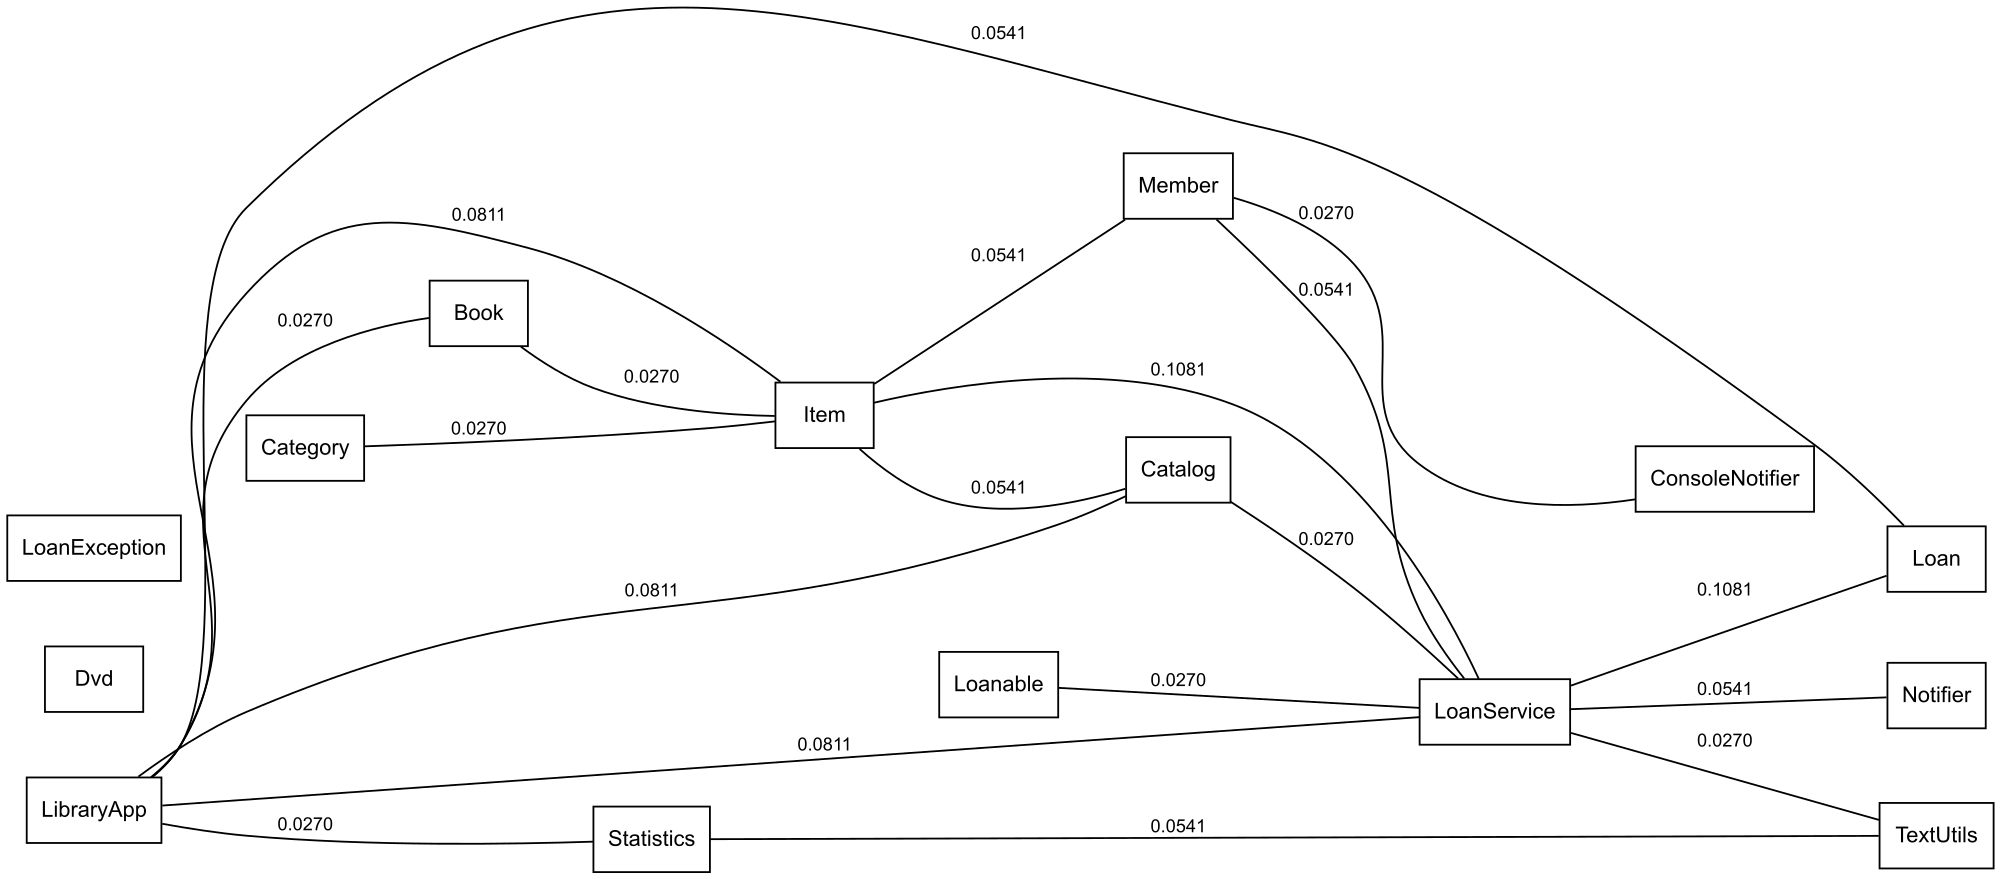
\includegraphics[width=\textwidth,height=0.8\textheight,keepaspectratio]{figures/coupling.png}
\caption{Graphe de couplage de référence : 15 sommets et 19 arêtes. Dvd et
LoanException sont explicitement conservées comme sommets isolés.}
Les noms courts sont utilisés sur cette figure pour la lisibilité ; Loan
désigne la classe membre LoanService.Loan. Les exports du programme conservent
les noms qualifiés.
\end{figure}

\section{B1 -- Clustering hiérarchique ascendant}
\subsection{Principe et implémentation}
Le service \texttt{ClusteringService} part du couplage A1. Initialement, chaque
classe forme un groupe. À chaque itération, nous fusionnons les deux groupes
actifs les plus similaires, jusqu'à obtenir un seul groupe. La similarité est
le lien moyen :
\[
S(G_1,G_2)=\frac{\sum_{a\in G_1}\sum_{b\in G_2}C(a,b)}{|G_1|\,|G_2|}.
\]
Les couples dont le couplage vaut zéro participent au dénominateur. Nous
recalculons les similarités depuis les couplages de classes, plutôt que de
prendre une moyenne non pondérée des anciennes similarités de groupes.
Cette implémentation privilégie la lisibilité : elle examine tous les couples
actifs et recalcule leurs valeurs à chaque étape. Sa complexité temporelle est
en $O(M^3)$, et le stockage de tous les membres des groupes peut atteindre
$O(M^2)$ ; cela convient aux petits projets du TP.

\subsection{Identifiants et égalités}
Les classes sont triées par nom qualifié et reçoivent les identifiants de 0 à
$M-1$. Les groupes créés reçoivent ensuite $M$, $M+1$, etc. Un couple est toujours
orienté du plus petit identifiant vers le plus grand. Nous cherchons d'abord le
maximum des similarités, puis retenons le premier couple dans l'ordre
lexicographique dont la valeur est à moins de $10^{-9}$ de ce maximum.
Cette recherche en deux passes évite de faire dépendre les égalités d'une
succession de comparaisons approchées. L'ordre d'addition est également stable,
car les membres sont triés.

Chaque fusion conserve les deux groupes réunis, le groupe créé et la similarité
au moment de la fusion. L'option \texttt{--output} écrit la trace UTF-8
\texttt{merges.csv} : étape, identifiants gauche et droit, nouvel identifiant,
similarité en pleine précision et membres du nouveau groupe. La représentation
explicite de l'arbre et son rendu sont décrits en B2.

\subsection{Résultats et validation}
Sur validation, les 15 classes donnent exactement \textbf{14 fusions}.
Les trois premières sont :
\begin{center}
\begin{tabular}{cllr}
Étape & Groupe gauche & Groupe droit & Similarité \\
\hline
1 & Item & LoanService & $4/37\simeq0{,}1081$ \\
2 & LibraryApp & Catalog & $3/37\simeq0{,}0811$ \\
3 & groupe 15 & groupe 16 & $9/148\simeq0{,}0608$
\end{tabular}
\end{center}
Le groupe 15 contient Item et LoanService ; le groupe 16 contient LibraryApp
et Catalog. Pour la troisième fusion, les quatre couples contribuent 3, 3, 2
et 1 arcs, d'où $(3+3+2+1)/(4\times37)=9/148$.
Les similarités ne remontent pas. Les deux dernières valent zéro : Dvd et
LoanException sont d'abord réunies, puis ce groupe rejoint les treize autres
classes. Une fusion à zéro termine l'arbre sans démontrer de dépendance entre
les groupes concernés.

Le micro jeu donne deux fusions de similarités $2/3$ puis $1/6$ ; la seconde
inclut bien le couple nul A--C dans sa moyenne.
La commande \texttt{mvn -o package} réussit avec \textbf{24 tests}, dont trois
tests B1. Ceux-ci vérifient les premières fusions, le nombre de fusions,
la partition des classes après chaque étape, l'union des membres, les
identifiants, la décroissance, les égalités avec tolérance et les cas vide,
singleton et sans relation.
Deux lancements complets sur notre TP1 ont donné la même sortie console et un
fichier \texttt{merges.csv} identique octet par octet.
\textbf{Le point de contrôle B1 est validé.}

\section{B2 -- Représentation du dendrogramme}
\subsection{Construction de l'arbre}
La classe \texttt{Dendrogram} transforme les fusions B1 en un arbre binaire
immuable. Chaque classe initiale devient une feuille. Pour chaque fusion,
nous retrouvons ses deux groupes actifs, créons leur parent et conservons
ses deux fils, son identifiant, ses membres et la similarité de fusion.
Une table indexée par identifiant permet de retrouver les sous-arbres.
Les deux fils sont retirés des groupes actifs et remplacés par le parent.
La construction refuse une fusion incohérente ou une trace incomplète.
Un jeu vide donne une racine absente ; une classe seule donne une feuille.

\subsection{Restitution}
Deux fichiers s'ajoutent aux exports précédents :
\begin{itemize}
\item \texttt{dendrogram.txt} : arbre indenté avec identifiants, noms qualifiés,
membres de chaque groupe et similarités en pleine précision ;
\item \texttt{dendrogram.dot} : arbre Graphviz avec les classes dans des
rectangles et les fusions dans des ellipses portant leur identifiant et leur
similarité à quatre décimales.
\end{itemize}
L'ordre chronologique des fusions reste explicite dans \texttt{merges.csv}.
Les images \texttt{dendrogram.svg} des jeux validation et mini ont été produites
par le moteur \texttt{dot} de Graphviz 16.1.0, via le paquet local
\texttt{@viz-js/viz} version 3.31.0. Un script reproductible est conservé dans
\texttt{tools/graphviz/render.mjs}. Cette dépendance sert uniquement au rendu ;
le programme Java et ses tests n'en dépendent pas.
La disposition est topologique, de la racine à gauche vers les feuilles à
droite : les distances dessinées ne mesurent pas les similarités. Celles-ci
se lisent sur les étiquettes. Le SVG de validation a également été converti
en PNG pour une inspection visuelle ; aucun chevauchement n'a été observé.

Depuis \texttt{TP2}, après le lancement Java avec \texttt{--output} :
\begin{verbatim}
npm ci --prefix tools/graphviz
node tools/graphviz/render.mjs output/validation output/mini
\end{verbatim}

\subsection{Validation et interprétation}
La commande \texttt{mvn -o package} réussit avec \textbf{26 tests}, dont deux
tests B2. Sur validation, l'arbre possède \textbf{15 feuilles et 14 nœuds
internes}, soit 29 nœuds et 28 liens parent--enfant. La racine G28 contient
les 15 classes, chacune une fois. Pour chaque nœud interne, les tests
vérifient que ses membres sont exactement l'union disjointe des membres de
ses deux fils. Les deux dernières fusions, G27 et G28, portent la similarité
zéro. Les tests couvrent aussi le micro jeu, le jeu vide, le singleton et
la stabilité des exports texte et DOT.

Les deux lancements Java ont produit leurs arbres texte et DOT ; les deux
images SVG ont été générées avec succès. L'arbre de validation montre un
regroupement progressif autour de Item et LoanService, puis des fusions à
faible similarité. Les classes isolées Dvd et LoanException sont réunies à
zéro, puis rattachées au reste. Ces rattachements complètent l'arbre sans
établir de relation d'appel. \textbf{Le point de contrôle B2 est validé.}
La sélection de modules par coupe est décrite en B3.
\begin{figure}[p]
\centering
\rotatebox{90}{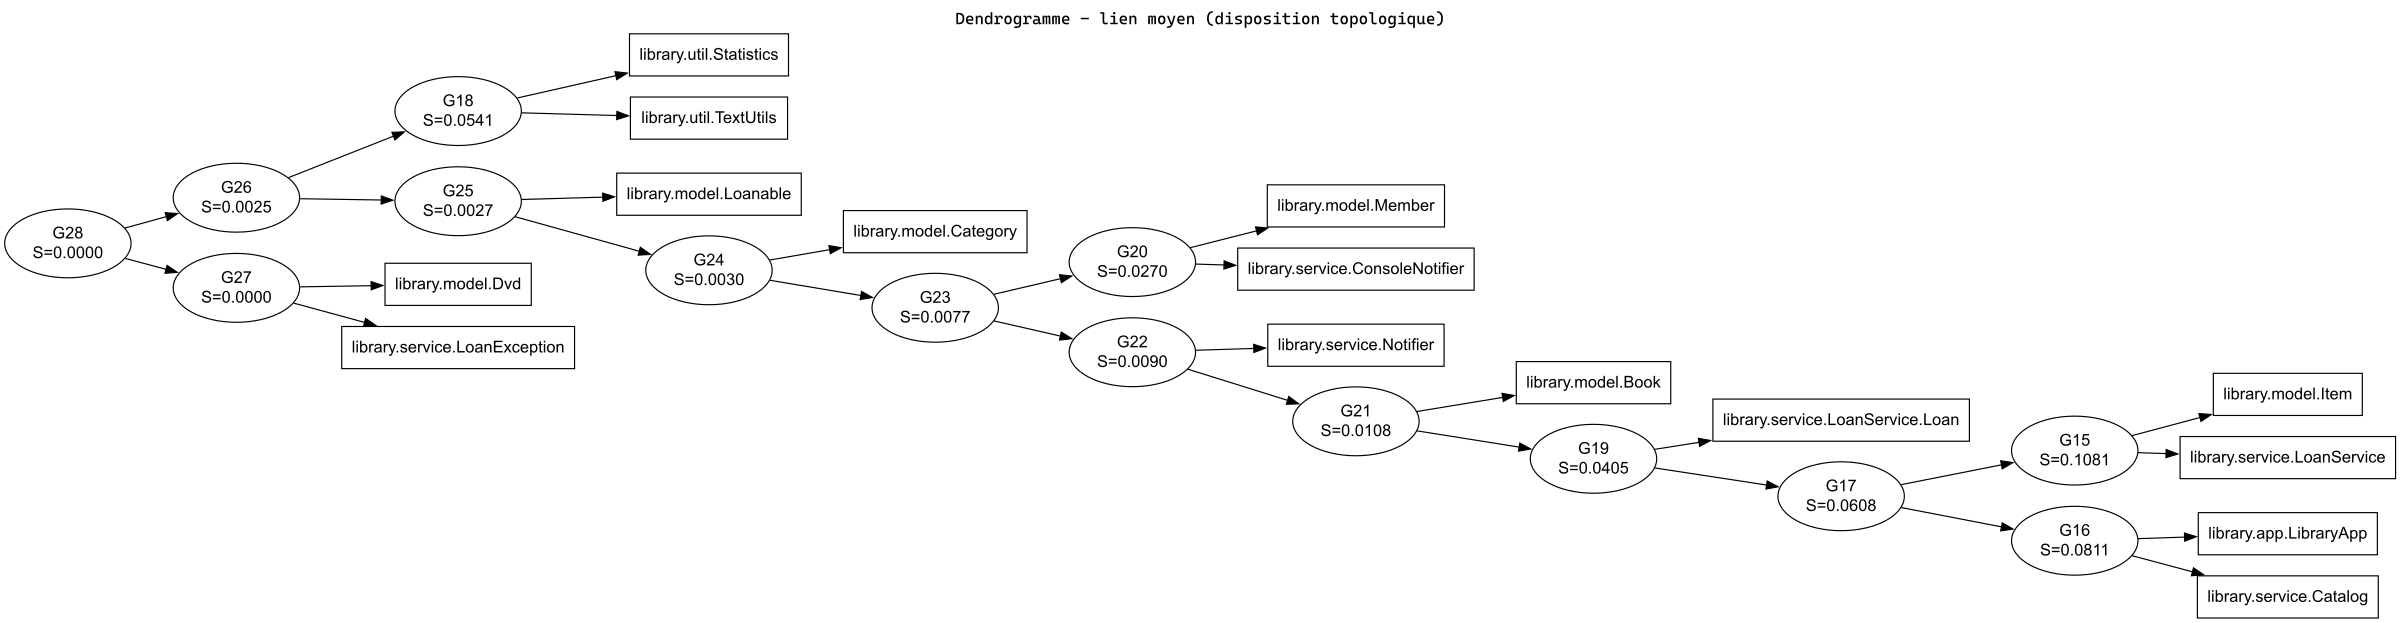
\includegraphics[width=0.88\textheight,height=0.85\textwidth,keepaspectratio]{figures/dendrogram.png}}
\caption{Dendrogramme de référence. Les similarités figurent sur les nœuds ;
la disposition topologique ne constitue pas une échelle métrique.}
\end{figure}

\section{B3 -- Coupe du dendrogramme et modules}
\subsection{Règle de coupe}
Le service \texttt{ModuleCut} parcourt l'arbre depuis la racine. Pour un groupe
$G$ d'au moins deux classes, il calcule le couplage interne moyen :
\[
\overline{C}(G)=\frac{\sum_{\{A,B\}\subseteq G,\ A\ne B}C(A,B)}{|G|(|G|-1)/2}.
\]
Chaque couple non orienté est compté une fois et les couples nuls participent
au dénominateur. Si $\overline{C}(G)>CP$, le groupe devient un module et le
parcours s'arrête dans cette branche. Sinon, nous descendons dans ses deux
fils. Une feuille devient toujours un module singleton ; sa moyenne est
indéfinie et affichée \texttt{NA}, et non zéro.
La comparaison au seuil est strictement supérieure, sans tolérance ajoutée.
Le seuil est fini, positif ou nul, et n'a pas de valeur par défaut.
Le test local de sélection s'écrit :
\begin{verbatim}
double mean = internalMean(coupling, node.members());
if (mean > threshold) {
    // Retenir ce sous-arbre et ne pas descendre dans ses fils.
}
\end{verbatim}

Le couplage interne moyen n'est pas la similarité de la fusion qui a créé le
groupe. Sur le micro jeu, la racine a une similarité de fusion de $1/6$, mais
une moyenne interne de $(2/3+1/3+0)/3=1/3$. À $CP=0{,}20$, elle est donc
retenue comme un seul module.

\subsection{Contrôle global et interface}
Après la coupe, nous vérifions que le nombre de modules ne dépasse pas
$\lfloor M/2\rfloor$. Nous ne modifions pas artificiellement les groupes
pour respecter cette limite. Une coupe trop fine est rejetée explicitement,
tout en conservant son résultat pour le diagnostic.
L'option \texttt{--cp} déclenche B3 ; son absence exécute les étapes jusqu'à B2
sans effectuer de coupe. Les options \texttt{--cp} et \texttt{--output} peuvent
être données dans les deux ordres. Le programme affiche chaque module avec
son identifiant de groupe, ses classes, son effectif et sa moyenne interne.
Avec \texttt{--output}, le fichier \texttt{modules.csv} conserve le seuil,
le statut de la coupe, la limite et les données de chaque module.
Le code de sortie est 0 si la coupe est acceptée, 3 si elle est rejetée,
1 pour des arguments invalides et 2 pour une erreur de traitement.

\subsection{Résultats mesurés}
Depuis \texttt{TP2/source}, nous avons exécuté, sur une seule ligne :
\begin{verbatim}
java -jar target/hai913i-tp2.jar --tp1 resources/validation
  --cp 0.025 --output ../output/cp-0.025
\end{verbatim}
La même commande a été exécutée avec les seuils 0,015 et 0,045 et des dossiers
de sortie distincts. Les résultats correspondent au sujet :
\begin{center}
\begin{tabular}{rrrrl}
CP & Modules & Limite & Plus grand module & Statut \\
\hline
0,015 & 4 & 7 & 11 classes & Acceptée \\
0,025 & 7 & 7 & 7 classes & Acceptée \\
0,045 & 10 & 7 & 5 classes & Rejetée
\end{tabular}
\end{center}
À $CP=0{,}025$, les sept modules sont :
\begin{itemize}
\item G22 : LibraryApp, Book, Item, Catalog, LoanService, LoanService.Loan et
Notifier ; moyenne $0{,}033462$ ;
\item G20 : Member et ConsoleNotifier ; moyenne $0{,}027027$ ;
\item G18 : Statistics et TextUtils ; moyenne $0{,}054054$ ;
\item quatre singletons : Category, Dvd, Loanable et LoanException.
\end{itemize}
Sur le micro jeu, $CP=0{,}20$ donne un module accepté et $CP=0{,}50$ donne deux
modules, au-delà de la limite de un : la coupe est rejetée.
Le rejet est un résultat de la règle de coupe et des contraintes, pas une
erreur de construction de l'arbre.

\subsection{Validation}
La commande \texttt{mvn -o package} réussit : \textbf{29 tests passent}, dont
trois tests B3. Ils vérifient les trois points de contrôle, l'appartenance de
chaque module à une branche, la partition complète des classes, les moyennes
au-dessus du seuil, les singletons et le cas d'égalité exacte au seuil.
Ils couvrent aussi le micro jeu, les seuils invalides, le jeu vide, un singleton
et un jeu sans relation. Pour une classe seule, l'application littérale de
$\lfloor M/2\rfloor=0$ rejette l'unique module. Les exécutions sur notre TP1
confirment les codes de sortie 0, 0 et 3 pour les trois seuils.
\textbf{Le point de contrôle B3 est validé.} L'interprétation architecturale
des regroupements est développée en B4.

\section{B4 -- Interprétation et critique des modules}
\subsection{Modules et paquetages}
Nous retenons la coupe à $CP=0{,}025$ comme base de discussion. Les sept modules
obtenus ne reproduisent pas les quatre paquetages du projet :
\begin{center}
\begin{tabular}{lrrrr}
Module & app & model & service & util \\
\hline
G22 (7 classes) & 1 & 2 & 4 & 0 \\
G20 (2 classes) & 0 & 1 & 1 & 0 \\
G18 (2 classes) & 0 & 0 & 0 & 2 \\
Category & 0 & 1 & 0 & 0 \\
Dvd & 0 & 1 & 0 & 0 \\
Loanable & 0 & 1 & 0 & 0 \\
LoanException & 0 & 0 & 1 & 0
\end{tabular}
\end{center}
Les colonnes désignent respectivement \texttt{library.app},
\texttt{library.model}, \texttt{library.service} et \texttt{library.util}.
G18 coïncide exactement avec le paquetage util : Statistics utilise les
méthodes \texttt{pad} et \texttt{repeat} de TextUtils pour produire son rapport.
Son couplage interne vaut $2/37$.

En revanche, G22 réunit le point d'entrée LibraryApp, Book et Item, ainsi que
Catalog, LoanService, LoanService.Loan et Notifier. Il traverse trois paquetages.
Les paquetages séparent ici des rôles (application, modèle métier, services),
alors que les appels réunissent les classes qui collaborent à l'exécution des
prêts. LibraryApp orchestre précisément ces collaborations. Ce décalage peut
donc traduire deux préoccupations différentes : organisation par responsabilités
et proximité des appels. Il ne suffit pas à démontrer une érosion architecturale.
Pour conclure à une telle érosion, il faudrait connaître les règles
d'architecture attendues et identifier leurs violations.

Le paquetage model est éclaté entre G22, G20 et trois singletons ; le paquetage
service est partagé entre G22, G20 et LoanException. Les frontières calculées
ne peuvent donc pas être adoptées telles quelles comme nouveau découpage des
paquetages. Elles constituent des pistes à examiner avec le rôle des classes.

\subsection{Pourquoi Dvd et LoanException sont isolées}
Dvd hérite de Item et est instanciée dans LibraryApp, mais ni l'héritage ni
l'expression \texttt{new} ne comptent dans la relation imposée. Son constructeur
appelle celui de Item, mais les appels de constructeurs sont également exclus
du graphe de méthodes retenu. Les méthodes déclarées dans Dvd ne produisent
aucun arc inter-classes dans les faits. Le graphe statique ne distribue pas
les appels polymorphes de Item vers toutes ses sous-classes possibles.
L'absence d'arête pour Dvd signifie donc une absence de relation \emph{mesurée},
pas une absence de dépendance métier ou structurelle.

LoanException est construite, levée et interceptée dans le scénario de prêts.
L'instanciation, la levée d'exception, les clauses \texttt{throws}/\texttt{catch}
et l'héritage de Exception sont hors de la relation comptée. Ces utilisations
ne créent donc pas d'arête inter-classes vers LoanException.

Dans le dendrogramme, ces deux classes rejoignent les autres à similarité zéro.
Pour les seuils positifs testés, la coupe descend jusqu'à leurs feuilles et
les conserve séparément. L'algorithme respecte ainsi sa définition ; la limite
vient d'abord du choix des dépendances observées.

\subsection{Un module discutable : Member et ConsoleNotifier}
G20 réunit une entité métier et un adaptateur d'affichage console appartenant
à deux paquetages différents. Les faits montrent un seul arc entre ces classes :
\texttt{ConsoleNotifier.send} appelle \texttt{Member.getName} pour composer le
message. Leur couplage vaut $1/37\simeq0{,}027027$, suffisamment pour retenir
leur branche avec $CP=0{,}025$.

Ce résultat est explicable par les calculs mais discutable comme choix de
conception : l'accès au nom d'un destinataire ne justifie pas nécessairement
de regrouper sa représentation métier avec un mécanisme d'affichage.
ConsoleNotifier implémente Notifier, mais cette relation n'est pas comptée.
Les appels de LoanService à \texttt{send} ciblent statiquement Notifier et
ne sont pas redirigés vers ConsoleNotifier. La chaîne voit donc un lien avec
Member et manque une partie du rôle architectural de l'implémentation.
L'ajout de l'implémentation d'interface est étudié en C2 ; il modifie les
branches du dendrogramme sans garantir un module commun aux deux types.

\subsection{Effet du seuil et choix retenu}
Les trois expériences de B3 montrent le compromis suivant :
\begin{itemize}
\item $CP=0{,}015$ donne 4 modules et respecte la limite, mais son module de
11 classes absorbe l'essentiel du système : le résultat est trop grossier
pour discuter précisément des responsabilités ;
\item $CP=0{,}025$ donne 7 modules, exactement la limite autorisée. Le noyau
de 7 classes reste large, mais les utilitaires et le couple Member--ConsoleNotifier
deviennent visibles séparément ;
\item $CP=0{,}045$ donne 10 modules. Le plus grand ne contient plus que
5 classes, mais cette coupe viole la contrainte $M/2$ et doit être rejetée.
\end{itemize}
Nous retenons donc \textbf{0,025 parmi les trois valeurs testées}, car il
préserve davantage de détail que 0,015 tout en respectant les contraintes.
Cela ne prouve ni son optimalité parmi tous les seuils possibles ni la qualité
architecturale de chacun de ses modules. Par exemple, G20 a une moyenne à peine
supérieure à ce seuil et reste sémantiquement discutable. Un seuil plus élevé
impose une moyenne plus forte, fait descendre la coupe et produit ici davantage
de modules ; il ne constitue pas à lui seul une amélioration architecturale.

\subsection{Limites : relation, liaison et seuil}
\paragraph{Relation comptée.}
La chaîne ne voit que les arcs d'appels statiquement résolus entre méthodes
du projet. Elle ignore notamment héritage, implémentation d'interface, types
des attributs et signatures, instanciations et exceptions. Elle ne mesure ni
la fréquence réelle à l'exécution, ni le coût d'un appel, ni son importance
métier. Compter les arcs plutôt que les sites donne le même poids à un couple
de méthodes appelé une fois ou plusieurs fois. La normalisation globale par
37 rend les valeurs et les seuils dépendants du projet : ajouter des relations
ailleurs changerait les valeurs même pour un couple inchangé.

\paragraph{Critère de liaison.}
Le lien moyen mesure une proximité moyenne, pas une responsabilité commune.
Les zéros diluent la similarité quand un groupe grossit ; quelques liens forts
ne suffisent donc pas toujours à entraîner une fusion précoce. Le regroupement
est glouton : les premières fusions ne sont jamais remises en cause. La règle
de départage garantit la reproductibilité mais ne donne aucune justification
sémantique au choix entre couples égaux. Les fusions finales à zéro servent
à terminer l'arbre et n'attestent pas d'une collaboration.

\paragraph{Seuil et coupe.}
CP ne change pas l'arbre ; il détermine les branches retenues. Les modules
doivent être des sous-arbres : une composition jugée préférable par un humain
peut donc être inaccessible à cette coupe. Le seuil est appliqué à une moyenne,
sans exiger que chaque couple interne soit fortement relié. Les singletons
échappent à ce critère, et la limite globale du nombre de modules peut rendre
une coupe trop fine inadmissible. Aucun seuil ne répare les dépendances absentes
du graphe initial.

En conclusion de cette étape, les résultats sont des \textbf{modules calculés},
à confronter à l'architecture attendue. Ils ne constituent pas automatiquement
des composants candidats dotés d'interfaces, et encore moins des composants
déployables ou des microservices. La cohérence du groupe utilitaire et les
limites illustrées par G20 justifient de comparer d'autres relations ou
critères dans la partie C. Les cinq points demandés en B4 sont traités à partir
des exports B3 et du code du projet de validation.

\section{C1 -- Comparaison du lien moyen et du lien simple}
\subsection{Extension et protocole}
Nous avons ajouté l'option \texttt{--linkage single}. Le lien moyen reste le
comportement par défaut et peut aussi être choisi par \texttt{--linkage average}.
Le lien simple définit la similarité par le meilleur couple :
\[
S_{\mathrm{simple}}(G_1,G_2)=\max_{a\in G_1,\,b\in G_2}C(a,b).
\]
Les deux variantes partagent la même boucle de regroupement, les identifiants,
la tolérance $10^{-9}$ et la règle de départage. Seule la fonction de liaison
change. Nous comparons donc les arbres sur le même graphe de 15 classes et
19 arêtes, sans changer le couplage, sa normalisation ou les faits d'entrée.
La coupe éventuelle conserve la moyenne interne et la règle stricte de B3,
même lorsque l'arbre a été construit par lien simple.

Les deux lancements suivants ont été exécutés depuis \texttt{TP2/source}
(chaque commande est à saisir sur une seule ligne) :
\begin{verbatim}
java -jar target/hai913i-tp2.jar --tp1 resources/validation
  --linkage average --cp 0.025 --output ../output/c1-average
java -jar target/hai913i-tp2.jar --tp1 resources/validation
  --linkage single --cp 0.025 --output ../output/c1-single
\end{verbatim}
Les dossiers distincts conservent les deux traces \texttt{merges.csv}, les arbres,
les modules et un fichier \texttt{linkage.txt}. Les titres des DOT identifient
le critère utilisé. Les deux SVG ont été générés avec le script Graphviz,
et celui du lien simple a été inspecté visuellement.

\subsection{Première divergence : deuxième fusion}
La première fusion est identique : Item et LoanService sont réunies à $4/37$.
Notons ce groupe $G=\{\mathrm{Item},\mathrm{LoanService}\}$.
À l'étape suivante, les variantes divergent :
\begin{itemize}
\item le lien moyen fusionne LibraryApp et Catalog à $3/37\simeq0{,}0811$ ;
\item le lien simple fusionne LoanService.Loan avec $G$ à
$4/37\simeq0{,}1081$.
\end{itemize}
La différence se vérifie sur les deux couples reliant Loan au groupe :
$C(\mathrm{Item},\mathrm{Loan})=0$ et
$C(\mathrm{LoanService},\mathrm{Loan})=4/37$.
Le lien moyen donne donc $(0+4/37)/2=2/37$, inférieur au $3/37$ du couple
LibraryApp--Catalog. Le lien simple retient le maximum $4/37$ et choisit Loan.
Ce premier écart vient du critère de liaison, pas d'un changement de graphe
ou d'une égalité départagée différemment.

En lien simple, LibraryApp et Catalog sont réunies à la troisième étape,
puis rejoignent le groupe Item--LoanService--Loan à la quatrième, à $3/37$.
En lien moyen, les deux paires initiales sont déjà réunies à la troisième
étape, à $9/148$, et Loan ne les rejoint qu'à la cinquième.
Les deux arbres possèdent 14 fusions et deux dernières similarités nulles,
mais leur ordre de fusion et leurs groupes intermédiaires diffèrent.

\subsection{Effet sur la coupe et interprétation}
À $CP=0{,}025$, les deux variantes donnent sept modules acceptés. Ce nombre
identique masque une composition différente. Le lien moyen conserve un noyau
de sept classes et le couple Member--ConsoleNotifier. En lien simple, Member
rejoint le noyau, qui contient huit classes et a une moyenne interne de
$0{,}028958$ ; ConsoleNotifier devient singleton. Le module utilitaire reste
Statistics--TextUtils, et Category, Dvd, Loanable et LoanException restent
singletons. Nous comparons les classes, et non les seuls identifiants de
groupes, dont le sens change avec l'ordre des fusions.

Le lien simple peut rattacher une classe à un groupe grâce à un seul lien fort,
même si elle est peu liée aux autres membres : c'est l'effet de chaînage.
Le lien moyen atténue cette attraction en tenant compte de tous les couples,
y compris les zéros. Aucune des deux fonctions ne garantit une responsabilité
métier commune. Le lien moyen demeure notre référence pour respecter les
conventions obligatoires et conserver la comparaison de B4 ; le lien simple
est présenté comme une variante explicitement nommée.

\subsection{Validation}
La commande \texttt{mvn -o package} réussit avec \textbf{32 tests}, dont trois
tests C1. Ils contrôlent la première fusion commune, la divergence à l'étape 2,
la composition du groupe obtenu, les 14 fusions, la racine complète,
la décroissance des similarités et la reproductibilité de la trace.
Les égalités et les cas vide, singleton et sans relation sont également testés.
Sur le micro jeu, la structure de l'arbre reste identique, mais la deuxième
similarité passe de $1/6$ en lien moyen à $1/3$ en lien simple : elle prend le
maximum de $C(A,C)=0$ et $C(B,C)=1/3$ plutôt que leur moyenne.
Les tests obligatoires du lien moyen continuent de passer.
\textbf{Le bonus C1 est réalisé et sa comparaison est documentée.}

\section{C2 -- Enrichissement des dépendances}
\subsection{Relations ajoutées et conventions}
L'option \texttt{--relations enriched} ajoute aux arcs d'appel deux relations
structurelles : l'héritage direct d'une classe et les interfaces directement
déclarées. Le modèle imposé reste disponible par \texttt{--relations calls},
qui est le comportement par défaut. Nous conservons le lien moyen pour isoler
l'effet de l'enrichissement de celui du bonus C1.

Nous exploitons les faits structurels déjà extraits par notre TP1. Son modèle
conserve une chaîne de superclasses ; l'adaptateur ne prend que la première,
avant de filtrer les types externes, afin de ne pas ajouter la fermeture
transitive de l'héritage. Les interfaces sont les interfaces directes du type.
Seuls les types déclarés dans le projet sont des extrémités admissibles.
Le contrat \texttt{InputFacts} expose ces faits neutres sans faire intervenir
JDT dans les calculs de couplage. Le chargeur CSV d'appels ne contient pas ces
informations : il refuse explicitement le mode enrichi, qui nécessite
\texttt{--tp1}. Le bloc JSON facultatif fourni n'est pas chargé par notre outil.

Chaque relation structurelle distincte compte pour une unité, comme un arc
de méthodes distinct ; ce choix de pondération est une convention du bonus,
pas une propriété universelle. Un couple peut cumuler appels et relation
structurelle. Si $s(A,B)$ est le nombre de relations structurelles entre les
deux classes, nous définissons :
\[
C_{\mathrm{enrichi}}(A,B)=\frac{r(A,B)+s(A,B)}{|E_{\mathrm{inter}}|+|S|}.
\]
Les relations structurelles sont dédupliquées par source, cible et nature.
Le sens est ensuite perdu pour le couplage, comme dans le modèle initial.
La somme sur les couples non orientés reste égale à 1.

\subsection{Relations observées et effet sur le graphe}
Quatre relations internes sont extraites : Book hérite de Item, Dvd hérite de
Item, Item implémente Loanable et ConsoleNotifier implémente Notifier.
Le dénominateur passe donc de 37 à 41. Le couple Book--Item existait déjà
par un appel ; il passe de $1/37$ à $2/41$. Trois nouvelles arêtes apparaissent,
portant le graphe de 19 à \textbf{22 arêtes} pour les mêmes 15 sommets.
Dvd n'est plus isolée : son couplage avec Item vaut $1/41$.
LoanException reste la seule classe isolée, car Exception est externe au
projet et nous ne comptons toujours ni instanciation ni levée d'exception.

Les cinq premières fusions gardent les mêmes groupes que la référence,
avec des valeurs renormalisées. La divergence structurelle apparaît à la
huitième fusion : Notifier rejoint le groupe Member--ConsoleNotifier en mode
enrichi, grâce au lien d'implémentation ajouté. Dans la référence, Notifier
rejoignait le noyau Item--LoanService. Loanable rejoint ensuite ce noyau par
sa relation avec Item. Dvd est rattachée à l'arbre à une similarité positive,
et seule la dernière fusion, avec LoanException, reste à zéro.

\subsection{Comparaison des modules et effet du dénominateur}
Les exécutions sur notre TP1, avec lien moyen dans tous les cas, donnent :
\begin{center}
\begin{tabular}{lrrrl}
Relation & Dénominateur & CP & Modules & Statut \\
\hline
Appels & 37 & 0,025 & 7 & Acceptée \\
Enrichie & 41 & 0,025 & 8 & Rejetée \\
Enrichie & 41 & $0,025\times37/41$ & 7 & Acceptée
\end{tabular}
\end{center}
À seuil numérique identique, le couple Member--ConsoleNotifier passe de
$1/37\simeq0{,}027027$ à $1/41\simeq0{,}024390$ et se sépare à la coupe.
Le noyau enrichi contient LibraryApp, Book, Item, Loanable, Catalog,
LoanService et LoanService.Loan ; Notifier n'en fait plus partie.
Le module utilitaire est conservé. Category, Dvd, Member, ConsoleNotifier,
LoanException et Notifier deviennent six singletons, d'où huit modules.
Le fait que Dvd ne soit plus isolée dans le graphe ne garantit donc pas
qu'elle fasse partie d'un module de plusieurs classes.

Pour examiner l'effet d'échelle, nous avons également testé
$CP'=0{,}025\times37/41\simeq0{,}022561$. Cet ajustement préserve la condition
sur les couples dont le numérateur ne change pas ; il ne restaure pas l'arbre
initial et ne constitue pas une recherche d'un seuil optimal.
La coupe donne alors sept modules : le noyau enrichi de sept classes, le
couple Member--ConsoleNotifier, Statistics--TextUtils et quatre singletons
Category, Dvd, LoanException et Notifier. Par rapport à la référence, Loanable
entre dans le noyau et Notifier en sort. Cette différence persiste malgré
l'ajustement d'échelle et reflète les nouvelles branches de l'arbre.

\subsection{Exécution et validation}
Depuis \texttt{TP2/source}, nous avons exécuté les commandes suivantes sur
une seule ligne chacune :
\begin{verbatim}
java -jar target/hai913i-tp2.jar --tp1 resources/validation
  --relations calls --cp 0.025 --output ../output/c2-calls
java -jar target/hai913i-tp2.jar --tp1 resources/validation
  --relations enriched --cp 0.025 --output ../output/c2-enriched
java -jar target/hai913i-tp2.jar --tp1 resources/validation
  --relations enriched --cp 0.0225609756097561
  --output ../output/c2-enriched-scaled
\end{verbatim}
Les exports incluent \texttt{relations.txt} pour identifier la variante et,
en mode enrichi, \texttt{structural-relations.csv} pour tracer les ajouts.
Les dendrogrammes SVG ont été générés dans les trois dossiers.
Les compteurs d'appels A0 restent 15 classes, 59 méthodes et 44 arcs : les
relations structurelles ne sont pas présentées comme de nouveaux appels.
Dans l'objet de couplage, le champ historique \texttt{interClassArcs}
désigne le nombre total de relations dans la variante enrichie ; la console
le présente comme le dénominateur des relations inter-classes.

La construction réussit avec \textbf{34 tests}, dont deux tests C2. Ils
vérifient les quatre relations exactes, le dénominateur 41, les 22 couples,
la symétrie, la somme égale à 1, les classes isolées, la partition et les
coupes de huit puis sept modules. Un test vérifie le refus des CSV sans
faits structurels. Les tests du modèle obligatoire continuent de passer.

\subsection{Bilan critique}
L'enrichissement rend visibles des liens ignorés en B4 : Dvd--Item et
ConsoleNotifier--Notifier notamment. Il ne produit pourtant pas automatiquement
une meilleure architecture. Il modifie simultanément les numérateurs, la
normalisation globale, l'ordre des fusions et les branches accessibles à la
coupe. L'égalité de poids entre un héritage et un arc d'appel reste discutable.
Les dépendances de signatures, d'attributs, d'instanciation et d'exceptions
restent absentes. Nous conservons donc les deux variantes explicitement
nommées et interprétons leurs écarts sans remplacer les conventions imposées.
\textbf{Le bonus C2 est réalisé et comparé au modèle de référence.}

\section{C3 -- Interface graphique interactive}
\subsection{Choix et architecture}
Nous avons ajouté une interface Swing, fournie avec le JDK, sans dépendance
supplémentaire. Elle constitue une seconde interface du même modèle Java :
\texttt{ExplorerPanel} réutilise \texttt{ClusteringService}, \texttt{Dendrogram}
et \texttt{ModuleCut}. Aucune formule de regroupement ou de coupe n'est
réimplémentée dans l'interface. Les faits sont chargés une fois par le lancement
habituel, puis transmis au panneau sous forme de couplage. Les manipulations
de l'interface s'effectuent sur le thread événementiel Swing.

\subsection{Interactions utiles}
L'interface propose les interactions suivantes :
\begin{enumerate}
\item \textbf{Navigation et inspection de l'arbre.} Les branches sont pliables.
Sélectionner un groupe affiche ses classes, son effectif, sa similarité de
fusion et son couplage interne moyen, explicitement distingués.
\item \textbf{Recherche de classe.} Une recherche partielle, insensible à la
casse, ouvre les chemins correspondants et sélectionne les feuilles trouvées.
Le nombre de résultats et l'absence de correspondance sont signalés.
\item \textbf{Modification de CP.} Le bouton d'application recalcule la coupe,
actualise la table des modules et affiche le respect ou le dépassement de
la limite $M/2$. Les seuils invalides sont refusés sans arrêter la fenêtre.
Sans seuil fourni, aucune coupe n'est calculée automatiquement.
\item \textbf{Inspection d'un module.} Cliquer une ligne de la table sélectionne
la branche correspondante et révèle sa composition dans le panneau de détail.
\item \textbf{Changement de liaison.} Le sélecteur permet de reconstruire
l'arbre en lien moyen ou simple et de recalculer la coupe au seuil saisi.
\end{enumerate}
Ces interactions permettent notamment de retrouver une classe isolée, de
comprendre la différence entre similarité de fusion et moyenne interne, et
d'observer le passage de sept à dix modules lorsque CP augmente de 0,025 à
0,045. Les vues restent synchronisées avec le modèle utilisé par la CLI.

\subsection{Lancement et périmètre}
Depuis \texttt{TP2/source}, lancer sur une seule ligne :
\begin{verbatim}
java -jar target/hai913i-tp2.jar --tp1 resources/validation
  --cp 0.025 --gui
\end{verbatim}
L'option peut être combinée avec \texttt{--csv}, \texttt{--linkage} et
\texttt{--relations enriched} (ce dernier nécessite toujours \texttt{--tp1}).
Les exports \texttt{--output} correspondent aux paramètres du lancement ;
les manipulations ultérieures dans la fenêtre ne les réécrivent pas.
La relation de dépendance est choisie au lancement, pas dans le panneau.
Il faut un environnement graphique ; Graphviz et un navigateur ne sont pas
nécessaires. L'arbre est présenté sous forme hiérarchique dépliable, et non
comme un dessin métrique du dendrogramme.

En mode graphique, une coupe rejetée est affichée dans la fenêtre, qui reste
ouverte pour corriger CP. Le lancement de la fenêtre retourne donc 0 lorsque
l'ouverture réussit ; le code 3 de rejet reste celui du mode CLI seul.
Les calculs interactifs synchrones conviennent au petit projet de validation ;
une analyse de grande taille demanderait un traitement en arrière-plan.

\subsection{Validation}
La construction réussit avec \textbf{36 tests}, dont deux tests C3 qui
manipulent les vrais composants Swing sur leur thread événementiel.
Ils vérifient la coupe initiale à sept modules, le passage à dix modules
rejetés, la recherche de Dvd et d'un nom absent, la sélection d'un module,
le refus de NaN, l'absence de seuil par défaut et le passage au lien simple
avec un noyau de huit classes. Le panneau a aussi été rendu hors écran et
inspecté visuellement ; la figure ci-dessous provient de ce panneau réel.
En complément, l'auteur a confirmé l'ouverture de la fenêtre native et le
dépliage de l'arbre. Les autres interactions n'ont pas encore fait l'objet
d'une vérification manuelle détaillée ; elles restent couvertes par les tests
automatisés décrits ci-dessus.

\begin{figure}[htbp]
\centering
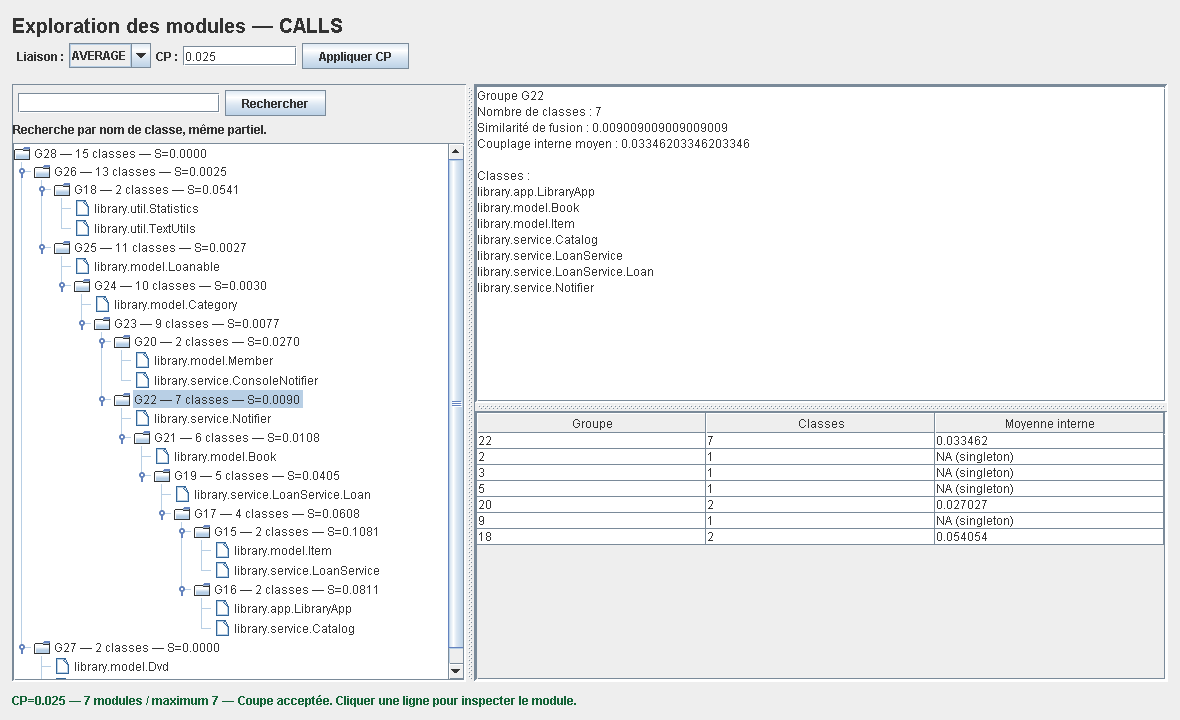
\includegraphics[width=\textwidth]{figures/explorer-c3.png}
\caption{Panneau Swing : arbre à gauche, groupe sélectionné en haut à droite,
modules en bas à droite et statut de coupe en bas. Rendu hors écran.}
\end{figure}
La figure conserve le rendu de contrôle du panneau Swing.
\textbf{Le bonus C3 est implémenté et ses interactions
sont couvertes par les tests.}

\section{C4 -- Extension à un second projet : non réalisée}
Je ne dispose pas d'un autre projet Java de taille modérée pour effectuer
les essais demandés en C4. Ce bonus n'a donc pas été réalisé. Les résultats
présentés concernent le projet de validation et le micro jeu fournis, ainsi
que leurs variantes de liaison et de dépendances. Ils ne permettent pas
d'affirmer que la méthode a été validée sur un second projet indépendant.

\section{Synthèse de validation et difficultés}
\begin{center}
\begin{tabular}{ll}
Étape & Résultat vérifié \\
\hline
A0 & 15 classes, 59 méthodes, 44 arcs ; micro jeu 3/5/4 \\
A1 & 7 arcs écartés, 37 retenus, 19 couples, somme 1 \\
A2 & 15 sommets, 19 arêtes, rechargement exact \\
B1 & 14 fusions, départage stable, trace reproductible \\
B2 & 15 feuilles, 14 nœuds internes, racine complète \\
B3 & 4, 7 et 10 modules pour CP=0,015 ; 0,025 ; 0,045 \\
B4 & Cinq points d'interprétation traités \\
C1 & Divergence dès la deuxième fusion \\
C2 & 4 relations ajoutées, 22 arêtes et dénominateur 41 \\
C3 & Recherche, inspection, coupe et liaison interactives \\
C4 & Non réalisé : aucun second projet disponible
\end{tabular}
\end{center}
La dernière suite complète comprend 36 tests réussis. La construction Maven
produit un JAR exécutable ; le micro jeu permet des vérifications manuelles.
Les comparaisons canoniques contrôlent le contenu des faits, pas seulement
les compteurs. Les tests de coupe contrôlent les partitions et les branches,
et ceux du graphe vérifient le rechargement sans perte de précision.

Les difficultés principales ont été la distinction entre arcs et sites,
les conventions différentes de nommage des constructeurs et le départage
déterministe des fusions. Le premier point est couvert par les comptages,
le second par une normalisation limitée aux tests de comparaison, le troisième
par des identifiants stables et une comparaison au maximum avec tolérance.
L'absence de Graphviz natif a été contournée par un outil local de rendu
WebAssembly, sans ajouter de dépendance au programme Java.

Les limites connues restent explicites : extraction statique partielle des
dépendances, choix de pondération du bonus C2, effet du dénominateur sur CP,
absence d'essai C4 et vérification manuelle encore partielle de la fenêtre native.
Les interactions Swing ont été testées automatiquement et le panneau a été
inspecté par rendu hors écran. Les manipulations graphiques ne réécrivent
pas les exports du lancement.

\section{Améliorations possibles et conclusion}
Une poursuite du travail pourrait comparer plusieurs pondérations des
relations structurelles, ajouter les dépendances d'instanciation et de
signatures, et évaluer la stabilité des modules sur plusieurs projets.
L'interface pourrait proposer l'export après interaction et des calculs en
arrière-plan pour les projets plus volumineux.

Le TP réalise la chaîne des faits aux modules et en rend les conventions
reproductibles. Le seuil 0,025 est retenu pour discuter la référence : il
conserve sept modules sans dépasser la limite, sans prétendre produire une
architecture optimale. Les bonus montrent que changer la liaison ou la
relation modifie les branches et les modules accessibles. L'interprétation
humaine reste indispensable pour distinguer une proximité d'appels, une
responsabilité métier et un véritable choix de conception.

\section{Usage de l'IA}
Un assistant d'intelligence artificielle a été utilisé pour répondre à des
questions, aider à la rédaction d'une partie du code, fournir des exemples
de code et contribuer à la mise en forme du rapport en \LaTeX.

\end{document}
